\chapter{Introduction}

This dissertation introduces a new approach to discovering context for photo annotation problems. The primary complexity of photo annotation problems lie in their large search spacesand the diversity of feature-based representations of images. Contextual information is used to prune this large search spaces with reduced dependency on image features. Once the search space has been reduced, the image features are used to select from the \textit{remaining} tags. For example, people with weak social ties do not co-occur often in photos, and by identifying one we can eliminate the other. In this case, we would say that social context is used to prune candidates in a face annotation problem.

Recently, there have been two changes in the scientific community which motivates us to take a fresh look at context. First, with mobile phones becoming the primary mode of photo taking, the nature of context has evolved from providing cues about tags, to the description of the world around a photo taking moment when a person was taking the photo. With the ever increasing amount of personal, social and public information, it is becoming harder to specify which subset of these would constitute the most interesting context for a given picture. Thus, it is not clear what data to consider context, and how do we combine them to form models of the real world which will allow photo annotation algorithms to reason what tags to assign various regions in a given photo.

More specifically, we address the problem of constructing computational representations of real world events from various heterogeneous data sources, to reason which parts of the search space can be pruned without hurting the overall performance of the annotation algorithm. We refer to such a representation as the \textbf{Context Network} of the photo. The network describes real-world events occurring in the environment, the entities participating in them, and their semantic inter-relationships.

\begin{figure}[t]
\centering
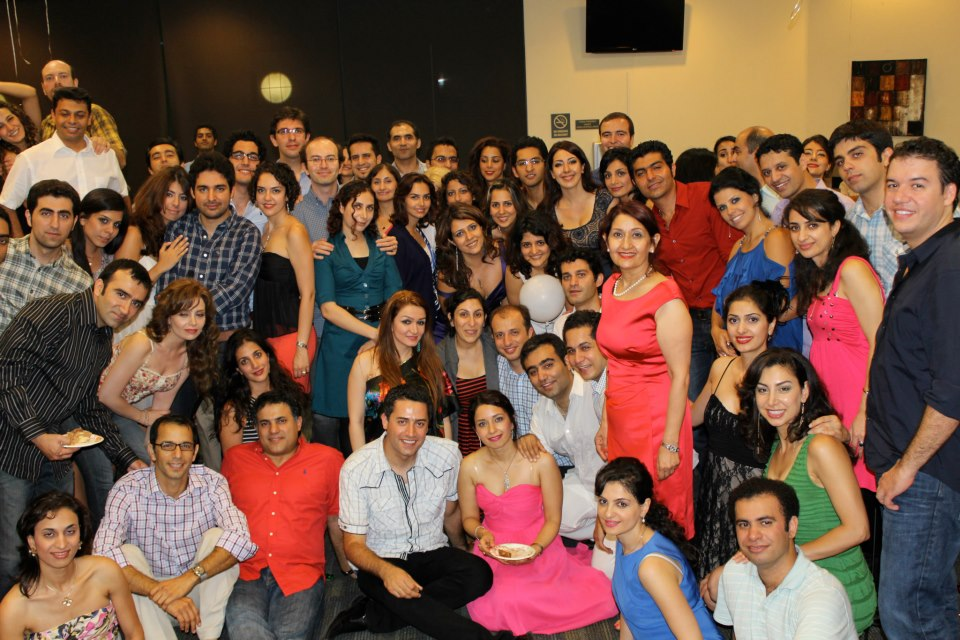
\includegraphics[width=0.8\textwidth]{media/chapter1/setarehetal}
\caption{Face tagging problems could be challenged by very large search spaces.}
\label{fig:people}
\end{figure}

\section{Importance of Context Discovery}

Computer science is moving towards solving real world problems. Social network analysis, medical diagnosis prediction, philanthropic engineering, monitoring public interests through real time communication networks, and situation-based advertising are some of the emerging applications in our area. The common requirement for all of them is to construct models of the real world events occurring in the world, who is participating in them and their attributes and relationships. A technology to construct such a model from various data sources currently available today can play a key role in the effective functioning of such systems.

For the purposes of this dissertation, we propose context discovery techniques in the light of photo annotation problems alone, but the technology and ideas are not tightly coupled with any singly media, and can be easily migrated to assist in solving any problem which requires models of real world events.

\section{Novelty}

Context has been used to address many multimedia problems \cite{henter2012tag, li2012fusing, naaman2005identity, o2009context,stone2008autotagging}. For example, time and location information or social network information from Facebook to solve the face recognition problem. We refer to such a direct dependency between the search space and a data source as \textbf{static linking}. Although these systems are meritorious in their own right, they suffer from the following drawbacks: they are tightly coupled with a few data sources, the unavailability of which would reduce the efficiency of the system, do not employ multiple sources, and therefore the \textbf{relations} between them. 

\begin{figure}[t]
\centering
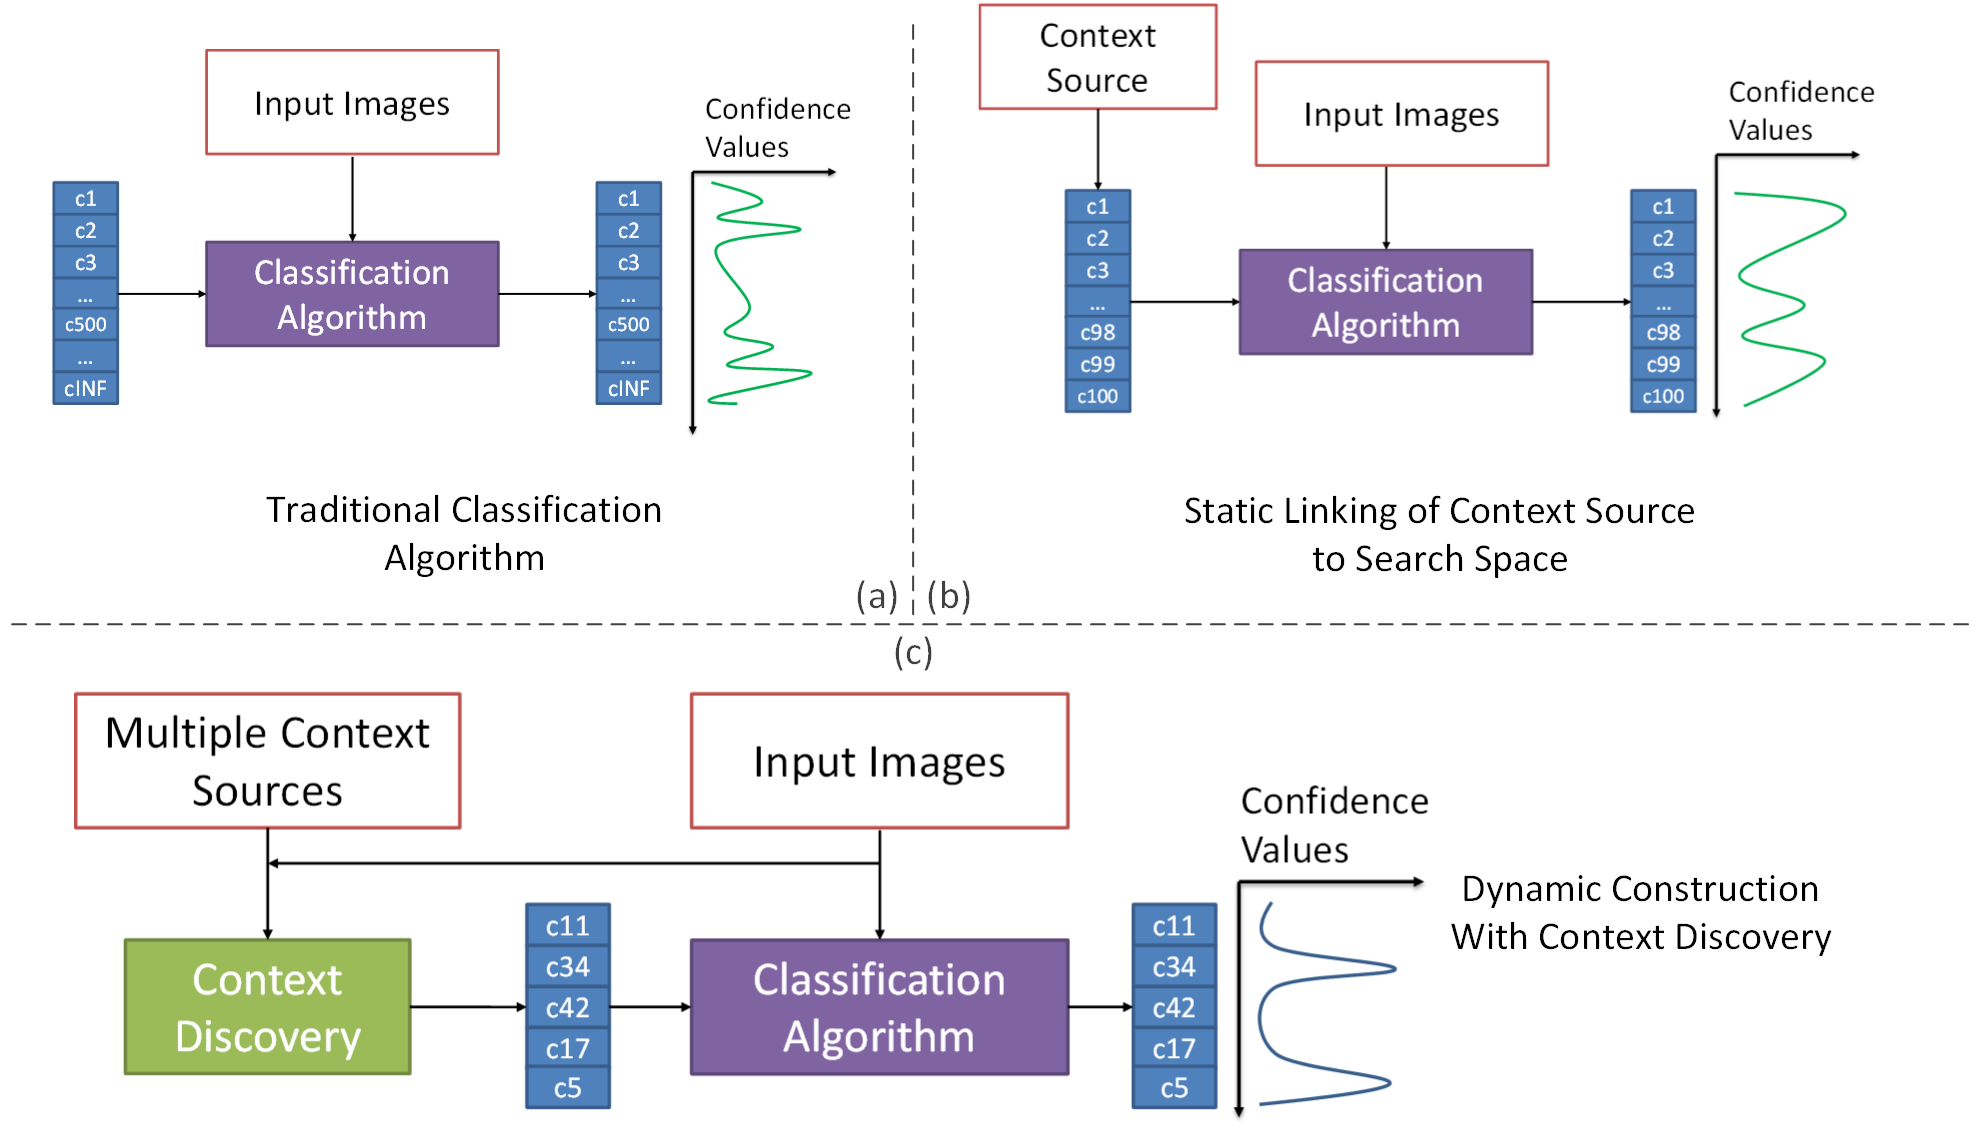
\includegraphics[width=0.85\textwidth]{media/with-without-cuenet-2.png}
\caption{The different approaches in search space construction for a multimedia annotation problem.}
\label{fig:with-without-cuenet}
\end{figure}

Figure \ref{fig:with-without-cuenet} shows the three major ways to prune search spaces in annotation systems. Figure \ref{fig:with-without-cuenet}(a) is one of the earliest system setups where the search spaces were manually constructed, and the focus was mainly on constructing smarter features to correctly classify feature sets \cite{turk1991eigenfaces, belhumeur1997eigenfaces}. Systems like \cite{stone2008autotagging} use a single source like Facebook to populate their search space based on some attributes of the input problem (in this case, the identity of the user). This restricted the search space but it is assumes that all relevant tags will be supplied from the context source, which is usually not correct.

This primary \uline{contribution} of this dissertation is a \textbf{\textit{progressive discovery}} algorithm to ingest information from various real world data sources to construct context networks containing the most relevant information for pruning the search space for the system. Examples of data sources include social media web services to provide information about events and entities like Facebook, Twitter; services which can be queried to find information about places like Yelp; Sensors on personal mobile phones, for example GPS which inform applications of the location of a person is present at any given point in time.

\section{Approach}

\textbf{What is progressive discovery?} Progressive discovery is an incremental process where knowledge of real world events and entities can be added to a given context network. Given a context network and multiple data sources describing events and entities, a progressive discovery algorithm will obtain new information from the sources and relate it to context network. By iteratively executing this algorithm, we can grow a context network until the data sources can provide no further information or the information in the network prunes the search space well enough for the AI problem to be fully solved.

The discussion in the following chapters on context networks and their discovery from various data sources will be presented in conjunction with an application to \textbf{tag faces in personal photos}. The face tagging algorithm, whose search space contains a few million entities attempts to solve a very hard problem. But if a real world model of the world existed, the search space which is relevant to this photo contains just the entities who are present within the field of view of the camera at the time the photo was captured. 

\section{Examples}
Here are two examples of dynamic linking. Figure \ref{fig:example-icmr-hidden} shows a photo of a person about to starting his presentation. Dynamic linking is done in three steps. First, the discovery algorithm proceeds to find the EXIF parameters of the photo, and associates the user with the photo. We call such an event where a photo is associated with its spatio-temporal attributes, a \texttt{photo-capture-event}. It signifies an event where the user is capturing an image with his camera. Second, these attributes are used to discover \textit{what is other events is the owner part of at this time}? Only those data sources are queried which can provide answers to this, and we obtain a response from a conference database saying that the owner was attending the ICMR conference at Dallas, Texas. Third, given this new conference event, the algorithm discovers what were the conference subevents (like keynotes, talks or break sessions) were occurring at this time. Finally, it finds that Mor Naaman and John Smith were speaker and host for the keynote talk going on that time. Given the two candidates, the face tagging algorithm proceeds to identify the correct tag, figure \ref{fig:example-icmr-show}.


\begin{figure}[ht]
\begin{minipage}[b]{0.45\linewidth}
\centering
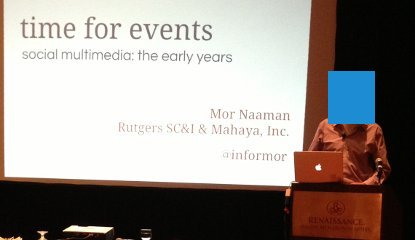
\includegraphics[width=\textwidth]{media/chapter1/icmr-keynote-2-hidden.jpg}
\caption{Who is in this photo?}
\label{fig:example-icmr-hidden}
\end{minipage}
\hspace{0.5cm}
\begin{minipage}[b]{0.45\linewidth}
\centering
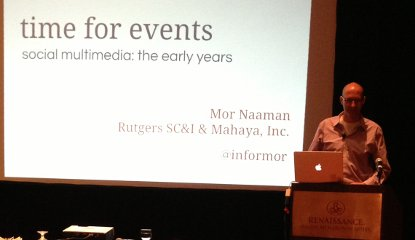
\includegraphics[width=\textwidth]{media/chapter1/icmr-keynote-2-show.jpg}
\caption{Mor Naaman at ICMR.}
\label{fig:example-icmr-show}
\end{minipage}
\end{figure}

Now, lets look at in photo in figure \ref{fig:example-kasturi-hidden}. Context discovery initiates the same way as in the above example, but after searching for events related to the owner in data sources, finds nothing. It proceeds to rank all known contacts according to location, and given that this photo was taken to the owner's workplace ranks colleagues higher than friends. The top 20 (an arbitrary constant) ranked candidates are passed to the face tagging algorithm which finds Ramesh Jain in the photo. But not the person to his right in the photo. But now, the \texttt{photo-capture-event} has an additional participant, Ramesh, whose calendar can be queried to find events in which he was participating. The calendar returns the entry ``Kasturi". The algorithm uses this term to find all Ramesh's contacts to find all people with first or last name ``Kasturi'', and finds his long time friend and colleague ``Rangachar Kasturi''. The face tagging algorithm is invoked with one candidate.

\begin{figure}[ht]
\begin{minipage}[b]{0.45\linewidth}
\centering
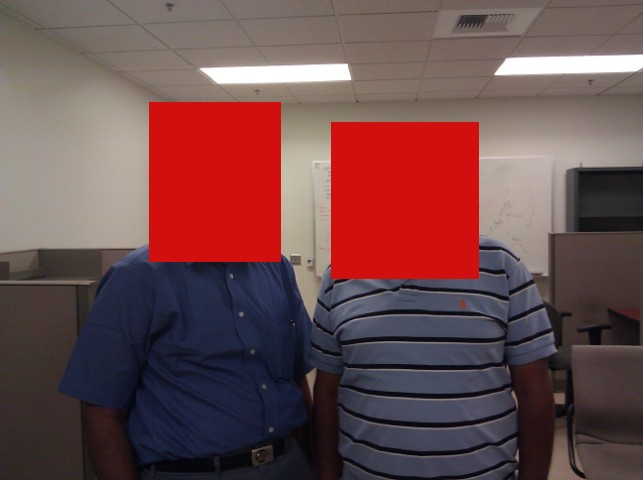
\includegraphics[width=\textwidth]{media/chapter1/kasturi-hidden.jpg}
\caption{Who is in this photo?}
\label{fig:example-kasturi-hidden}
\end{minipage}
\hspace{0.5cm}
\begin{minipage}[b]{0.45\linewidth}
\centering
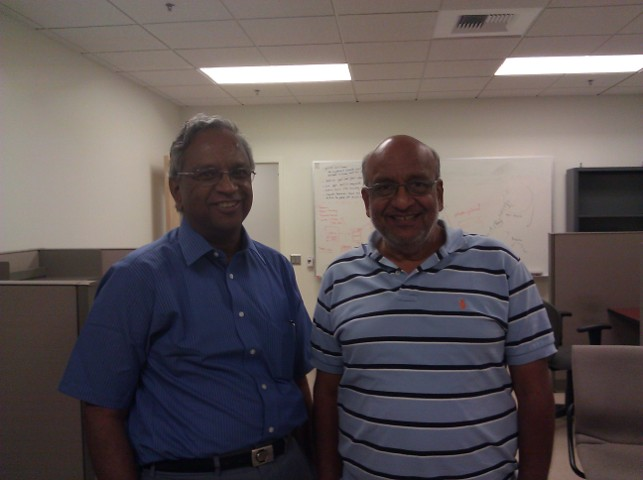
\includegraphics[width=\textwidth]{media/chapter1/kasturi-show.jpg}
\caption{Kasturi and Jain.}
\label{fig:example-kasturi-show}
\end{minipage}
\end{figure}

In this first run, the algorithm linked only to a conference database, whereas in the second case, it used spatial information, personal calendar and contact information. In the later chapters, we will present techniques to represent and link context in a systematic manner.

\section{Overview}
This dissertation is organized into the following chapters. Chapter 2 provides an overview of context, how context has been used to address problems in various scientific disciplines and how we use context in our specific personal photo tagging application. Chapter 3 describes the related work in computer science, and how this work is informed by them. Chapter 4 describes our context discovery framework, how it models various data sources, and how our progressive discovery algorithm constructs models for real world problems. We facilitate this discussion with an example real world application to tag faces of people in personal photos. Chapter 5 analyzes the algorithmic complexity of different parts of the system, and provides experiments to verify the competence and performance of the system. We also present experiments to confirm the efficacy of our approach in the light of the real world application. Finally, chapter 6 attempts to describe the future possibilities of using context discovery in computer science.

% Chapters 6 and 7 describe two extensions to the CueNet framework to solve problems of missing context and that of source selection. 

%% \section{Terminology}
%% Before starting the discussion on Context Networks, it is necessary to include a short note on terminology to avoid any ambiguities. We use the word `Object' to collectively refer to events and entities. An entity includes persons, places in the world, for example `Starbucks, UC Irvine', `The Eiffel Tower, Paris, France', or organizations, for example `Google Inc', `Royal Society of London'. The term `object' has been used in literature to refer to things which have no temporal properties. But, in our discussion, an `object' could imply an event which exhibits temporal properties.

% \begin{figure}[h]
% \centering
% 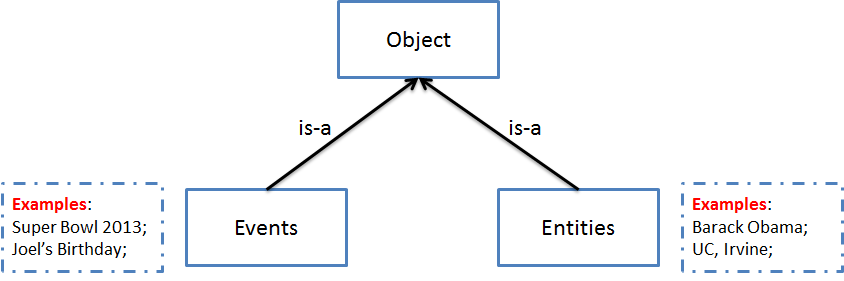
\includegraphics[width=0.75\textwidth]{media/chapter1/terminology.png}
% \caption{Objects, Events and Entities.}
% \label{fig:terminology}
% \end{figure}


% \begin{figure}[ht]
% \begin{minipage}[b]{0.45\linewidth}
% \centering
% 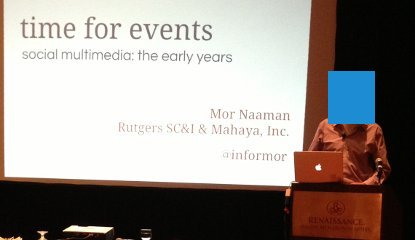
\includegraphics[width=\textwidth]{media/chapter1/icmr-keynote-2-hidden.jpg}
% \caption{Who is in this photo?}
% \label{fig:example-icmr-hidden}
% \end{minipage}
% \hspace{0.5cm}
% \begin{minipage}[b]{0.45\linewidth}
% \centering
% 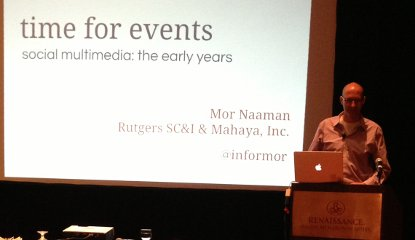
\includegraphics[width=\textwidth]{media/chapter1/icmr-keynote-2-show.jpg}
% \caption{Mor Naaman at ICMR.}
% \label{fig:example-icmr-show}
% \end{minipage}
% \end{figure}
